\documentclass[prc,twocolumn,amssymb,amsmath,showpacs,superscriptaddress]{revtex4}
\usepackage{epsfig,subfigure,graphicx,dcolumn,bm,latexsym}
\bibliographystyle{apsrev}

\def\Journal#1#2#3#4{{#1} {\bf #2}, #3 (#4)}
\def\NIMR{Nucl. Instrum. Methods Phys. Res. A}
\def\NIMB{Nucl. Instrum. Methods Phys. Res. B}
\def\ADNDT{At. Data Nucl. Data Tables}
\def\NPA{Nucl. Phys.}
\def\CPC{Comput. Phys. Commun.}
\def\PLB{Phys. Lett. B}
\def\PRL{Phys. Rev. Lett.}
\def\PRep{Phys. Rep.}
\def\PRC{Phys. Rev. C}
\def\PR{Phys. Rep.}
\def\ZPA{Z. Phys. A}
\def\EPJA{Eur. J. Phys. A}
\def\MPL{Mod. Phys. Lett. A}
\def\ARNPS{Annu. Rev. Nucl. Part. Sci.}
\def\RPP{Rep. on Progr. in Phys.}
\def\MFMDVS{Mat. Fys. Medd. Dan. Vid. Selsk.}
\def\ActaB{Acta Phys. Pol.}

\begin{document}

\title{$^{108}$Sn studied with intermediate-energy Coulomb
excitation}

\author{A.~Banu}
\affiliation{Gesellschaft f{\"u}r Schwerionenforschung (GSI),
D-64291 Darmstadt, Germany} \affiliation{Institut f{\"u}r
Kernphysik, Universit{\"a}t Mainz, D-55099 Mainz, Germany}
\author{J.~Gerl}
\affiliation{Gesellschaft f{\"u}r Schwerionenforschung (GSI),
D-64291 Darmstadt, Germany}
\author{C.~Fahlander}
\affiliation{Department of Physics, Lund University, S-22100 Lund,
Sweden}
\author{M.~G\'{o}rska}
\affiliation{Gesellschaft f{\"u}r Schwerionenforschung (GSI),
D-64291 Darmstadt, Germany}
\author{H.~Grawe}
\affiliation{Gesellschaft f{\"u}r Schwerionenforschung (GSI),
D-64291 Darmstadt, Germany}
\author{T.R.~Saito}
\affiliation{Gesellschaft f{\"u}r Schwerionenforschung (GSI),
D-64291 Darmstadt, Germany}
\author{H.-J.~Wollersheim}
\affiliation{Gesellschaft f{\"u}r Schwerionenforschung (GSI),
D-64291 Darmstadt, Germany}
\author{E.~Caurier}
\affiliation{IReS, F-67037 Strasbourg Cedex 2, France}
\author{T.~Engeland}
\affiliation{Department of Physics and Center of Mathematics for
Applications, University of Oslo, N-0316 Oslo, Norway}
\author{A.~Gniady}
\affiliation{IReS, F-67037 Strasbourg Cedex 2, France}
\author{M.~Hjorth-Jensen}
\affiliation{Department of Physics and Center of Mathematics for
Applications, University of Oslo, N-0316 Oslo, Norway}
\author{F.~Nowacki}
\affiliation{IReS, F-67037 Strasbourg Cedex 2, France}
\author{T.~Beck}
\affiliation{Gesellschaft f{\"u}r Schwerionenforschung (GSI),
D-64291 Darmstadt, Germany}
\author{F.~Becker}
\affiliation{Gesellschaft f{\"u}r Schwerionenforschung (GSI),
D-64291 Darmstadt, Germany}
\author{P.~Bednarczyk}
\affiliation{Gesellschaft f{\"u}r Schwerionenforschung (GSI),
D-64291 Darmstadt, Germany} \affiliation{The Henryk
Niewodnicza\'{n}ski Institute of Nuclear Physics, PAN, 31-342
Krak{\'o}w, Poland}
\author{M.A.~Bentley}
\affiliation{Department of Physics, University of York,
Heslington, York YO10 5DD, UK}
\author{A.~B\"{u}rger}
\affiliation{Helmholtz-Institut f\"{u}r Strahlen- und Kernphysik,
Universit\"{a}t Bonn, D-53115 Bonn, Germany}
\author{F.~Cristancho}
\altaffiliation{On leave of absence from Universidad Nacional de
Colombia, Bogota, Colombia} \affiliation{Department of Physics,
Lund University, S-22100 Lund, Sweden}
\author{G.~de Angelis}
\affiliation{INFN Laboratori Nazionali di Legnaro, I-35020
Legnaro, Italy}
\author{Zs.~Dombr{\'a}di}
\affiliation{Institute of Nuclear Research of the Hungarian
Academy of Sciences, H-4001 Debrecen, Hungary}
\author{P.~Doornenbal}
\affiliation{Gesellschaft f{\"u}r Schwerionenforschung (GSI),
D-64291 Darmstadt, Germany} \affiliation{Institut f\"{u}r
Kernphysik, Universit\"{a}t zu K{\"o}ln, D-50937 K{\"o}ln,
Germany}
\author{H.~Geissel}
\affiliation{Gesellschaft f{\"u}r Schwerionenforschung (GSI),
D-64291 Darmstadt, Germany}
\author{J.~Gr\c{e}bosz}
\affiliation{Gesellschaft f{\"u}r Schwerionenforschung (GSI),
D-64291 Darmstadt, Germany} \affiliation{The Henryk
Niewodnicza\'{n}ski Institute of Nuclear Physics, PAN, 31-342
Krak{\'o}w, Poland}
\author{G.~Hammond}
\altaffiliation[Present address: ]{Department of Physics,
University of York, Heslington, York, UK} \affiliation{Department
of Physics, University of Keele, Keele, Staffordshire ST5 5BG, UK}
\author{M.~Hellstr\"{o}m}
\altaffiliation[Present address: ]{Department of Physics, Lund
University, Lund, Sweden} \affiliation{Gesellschaft f{\"u}r
Schwerionenforschung (GSI), D-64291 Darmstadt, Germany}
\author{J.~Jolie}
\affiliation{Institut f\"{u}r Kernphysik, Universit\"{a}t zu
K{\"o}ln, D-50937 K{\"o}ln, Germany}
\author{I.~Kojouharov}
\affiliation{Gesellschaft f{\"u}r Schwerionenforschung (GSI),
D-64291 Darmstadt, Germany}
\author{N.~Kurz}
\affiliation{Gesellschaft f{\"u}r Schwerionenforschung (GSI),
D-64291 Darmstadt, Germany}
\author{R.~Lozeva}
\altaffiliation[Present address: ]{Faculty of Physics, University
of Sofia, Sofia, Bulgaria} \affiliation{Gesellschaft f{\"u}r
Schwerionenforschung (GSI), D-64291 Darmstadt, Germany}
\author{S.~Mandal}
\altaffiliation[Present address: ]{University of Delhi, New Delhi,
India} \affiliation{Gesellschaft f{\"u}r Schwerionenforschung
(GSI), D-64291 Darmstadt, Germany}
\author{N.~M\u{a}rginean}
\affiliation{INFN Laboratori Nazionali di Legnaro, I-35020
Legnaro, Italy}
\author{S.~Muralithar}
\altaffiliation[Present address: ]{Nuclear Science Center, New
Delhi, India} \affiliation{Gesellschaft f{\"u}r
Schwerionenforschung (GSI), D-64291 Darmstadt, Germany}
\author{J.~Nyberg}
\affiliation{Department of Radiation Sciences, Uppsala University,
SE-75121 Uppsala, Sweden}
\author{J.~Pochodzalla}
\affiliation{Institut f{\"u}r Kernphysik, Universit{\"a}t Mainz,
D-55099 Mainz, Germany}
\author{W.~Prokopowicz}
\affiliation{Gesellschaft f{\"u}r Schwerionenforschung (GSI),
D-64291 Darmstadt, Germany} \affiliation{The Henryk
Niewodnicza\'{n}ski Institute of Nuclear Physics, PAN, 31-342
Krak{\'o}w, Poland}
\author{P.~Reiter}
\affiliation{Institut f\"{u}r Kernphysik, Universit\"{a}t zu
K{\"o}ln, D-50937 K{\"o}ln, Germany}
\author{D.~Rudolph}
\affiliation{Department of Physics, Lund University, S-22100 Lund,
Sweden}
\author{C.~Rusu}
\affiliation{INFN Laboratori Nazionali di Legnaro, I-35020
Legnaro, Italy}
\author{N.~Saito}
\affiliation{Gesellschaft f{\"u}r Schwerionenforschung (GSI),
D-64291 Darmstadt, Germany}
\author{H.~Schaffner}
\affiliation{Gesellschaft f{\"u}r Schwerionenforschung (GSI),
D-64291 Darmstadt, Germany}
\author{D.~Sohler}
\affiliation{Institute of Nuclear Research of the Hungarian
Academy of Sciences, H-4001 Debrecen, Hungary}
\author{H.~Weick}
\affiliation{Gesellschaft f{\"u}r Schwerionenforschung (GSI),
D-64291 Darmstadt, Germany}
\author{C.~Wheldon}
\altaffiliation[Present address: ]{Hahn-Meitner-Institut Berlin,
Berlin, Germany} \affiliation{Gesellschaft f{\"u}r
Schwerionenforschung (GSI), D-64291 Darmstadt, Germany}
\author{M.~Winkler}
\affiliation{Gesellschaft f{\"u}r Schwerionenforschung (GSI),
D-64291 Darmstadt, Germany}

\date{\today}

\begin{abstract}
The unstable neutron-deficient $^{108}$Sn isotope has been studied
in inverse kinematics by intermediate-energy Coulomb excitation
using the RISING/FRS experimental set-up at GSI. This is the
highest-Z nucleus studied so far with this method. Its reduced
transition probability B(E2;0$_{\text{g.s.}}^{+}$$\to$2$_{1}^{+})$
has been measured for the first time. The extracted B(E2) value of
$0.230(57)\ \text{e}^2\text{b}^2$ has been determined relative to
the known value in the stable $^{112}$Sn isotope. The result is
discussed in the framework of recent large-scale shell model
calculations performed with realistic effective interactions. The
role of particle-hole excitations of the $^{100}$Sn core and of
the $Z=50$ shell gap for the E2 polarization are investigated.
\end{abstract}

\pacs{21.10.-k, 25.70.De, 23.20.Js, 21.60.Cs}

\maketitle

The structure of nuclei far from $\beta$-stability is currently a
key topic of research, both experimentally and theoretically. The
emphasis is put on phenomena such as shell evolution,
proton-neutron interaction, and changes of collective properties.
A key question in nuclear structure physics is whether the shell
closures known close to the valley of stability are preserved when
approaching the limits of nuclear existence. Towards the proton
drip line due to the confinement of protons by the Coulomb barrier
and/or the vicinity of the $N=Z$ line, changes in shell structure
as well as collectivity are expected to be driven exclusively by
the monopole drift \cite{ots01,gra04} of single-particle states
and the proton-neutron interaction between identical shell model
orbitals \cite{naz95}. Hence, core polarization studied in spin
(M1, Gamow-Teller) and shape (E2) response, proton-neutron
pairing, and isospin symmetry are appealing nuclear structure
investigations. In this respect, the heaviest proton bound $N=Z$
doubly-magic nucleus $^{100}$Sn and its neighbors provide a
principle test ground. Information on quadrupole polarization of
the magic core can be inferred from the energy of the first
excited 2$^+$ states and their E2 transition rates to the ground
state. Experimentally, the nuclear properties of $^{100}$Sn are
only indirectly known \cite{gor97,gor98,lip98,bla04}, although its
existence has already been confirmed \cite{lew94,sch94}. \\
The Sn isotopes between the $N=50$ and $82$ shell closures provide
the longest chain of semi-magic nuclei accessible to nuclear
structure studies, both in the neutron valence space of a full
major shell and with emphasis on excitations of the $Z=50$ core.
The B(E2;0$^+_{\text{g.s.}}$$\to$2$^+_1$) value is most sensitive
to details of shell structure and E2 core polarization. However,
the existence of higher lying isomeric states in the tin isotopes
hampers a direct measurement of the lifetime of the $2^{+}_{1}$
states by standard Doppler methods (DSAM, RDM) and the very short
lifetimes of the $2^{+}_{1}$ states are not accessible to
electronic timing methods. Therefore, a Coulomb excitation
measurement is the only way to obtain this nuclear structure
information. Until recently only the
B(E2;0$^+_{\text{g.s.}}$$\to$2$^+_1$) values of the stable
$^{112-124}$Sn nuclei were measured in subbarrier Coulomb
excitation~\cite{ram01}.

In the following, we report on the first intermediate-energy
Coulomb excitation experiment performed on the $^{108,112}$Sn
isotopes using the RISING/FRS set-up \cite{wol05}. A primary beam
of $^{124}$Xe at $700\ \text{MeV/nucleon}$ energy and an average
intensity of $6 \times 10^{7}\ \text{s}^{-1}$, delivered by the
SIS accelerator at GSI, impinged on a $4\ \text{g/cm}^{2}$ $^9$Be
production target located at the entrance of the fragment
separator (FRS)~\cite{gei92}. The Sn isotopes were produced via
projectile fragmentation. Secondary beams were separated by the
FRS operated in achromatic optics mode, and identified on an
event-by-event basis by coincidence measurements of energy loss in
an ionization chamber, magnetic rigidity, and time-of-flight using
two scintillator detectors. The trajectories of the projectiles
were tracked with two multiwire proportional chambers. A
wedge-shaped aluminium degrader with thickness of $4.59\
\text{g/cm}^{2}$ and $4.83\ \text{g/cm}^{2}$ for the $^{108}$Sn
and $^{112}$Sn fragment settings, respectively, was placed at the
middle focal plane of the FRS. This allowed an optimized
separation of the fragments of interest amounting in both cases to
$\simeq 60 \%$ of the secondary beam cocktail. At the final focal
plane of the fragment separator, a secondary $^{197}$Au target was
placed with a thickness of $386\ \text{mg/cm}^{2}$. The
$^{108,112}$Sn nuclei impinging on the gold target at $142\
\text{MeV/nucleon}$ and $147\ \text{MeV/nucleon}$ energies,
respectively, were mainly excited by means of electromagnetic
interaction. Gamma rays in coincidence with projectile residues
were detected by the 15 RISING Ge-Cluster detectors
\cite{sim97,wol05}. The position sensitive detector array CATE
\cite{loz05}, consisting of $3 \times 3$ Si-CsI(Tl) modular
$\Delta$E-E telescopes, and covering an opening angle of $58\
\text{mrad}$, was placed at $1426\ \text{mm}$ downstream from the
secondary target. It served for the reaction channel selection as
well as for the scattering angle determination.

At intermediate energies, a Coulomb excitation measurement is an
experimental challenge because of intense atomic background
radiation and relativistic Doppler effects. Previously, the method
has been applied to nuclei with $Z \leq 30$ only. The 15 RISING
Ge-Cluster detectors were positioned at forward angles with a
small opening angle of $3^{\circ}$ (for each single crystal) in
order to maximize the effective solid angle affected by the
Lorentz boost, while at the same time minimizing the Doppler
broadening. This allowed an energy resolution of $3 \%$ to be
achieved for projectile residue velocities of $\cong 0.46 c$. To
suppress the atomic background radiation, each Ge-Cluster detector
was surrounded on the side by a lead sheet of $2\ \text{mm}$
thickness, and its front face was shielded by a combination of Pb,
Sn and Al absorbers of $5\ \text{mm}$ thickness. In the analysis,
an add-back procedure (applied to all 7 crystals within a
Ge-Cluster) as well as Doppler-shift correction were performed
event by event. For technical reasons (see Ref.~\cite{ban05} for
details) only five of the RISING Ge-Cluster detectors were
suitable for the off-line data analysis. The top panel in
Fig.~\ref{fig:Sn_peaks} shows the Doppler corrected energy
spectrum of the excited $^{112}$Sn, with the $\gamma$-ray line of
interest at $1257\ \text{keV}$.  The bottom panel shows the
corresponding spectrum for $^{108}$Sn with the $\gamma$-ray line
at $1206\ \text{keV}$.

\begin{figure}[htb]%
\centering
\subfigure{%
\resizebox{0.35\textwidth}{!}{%
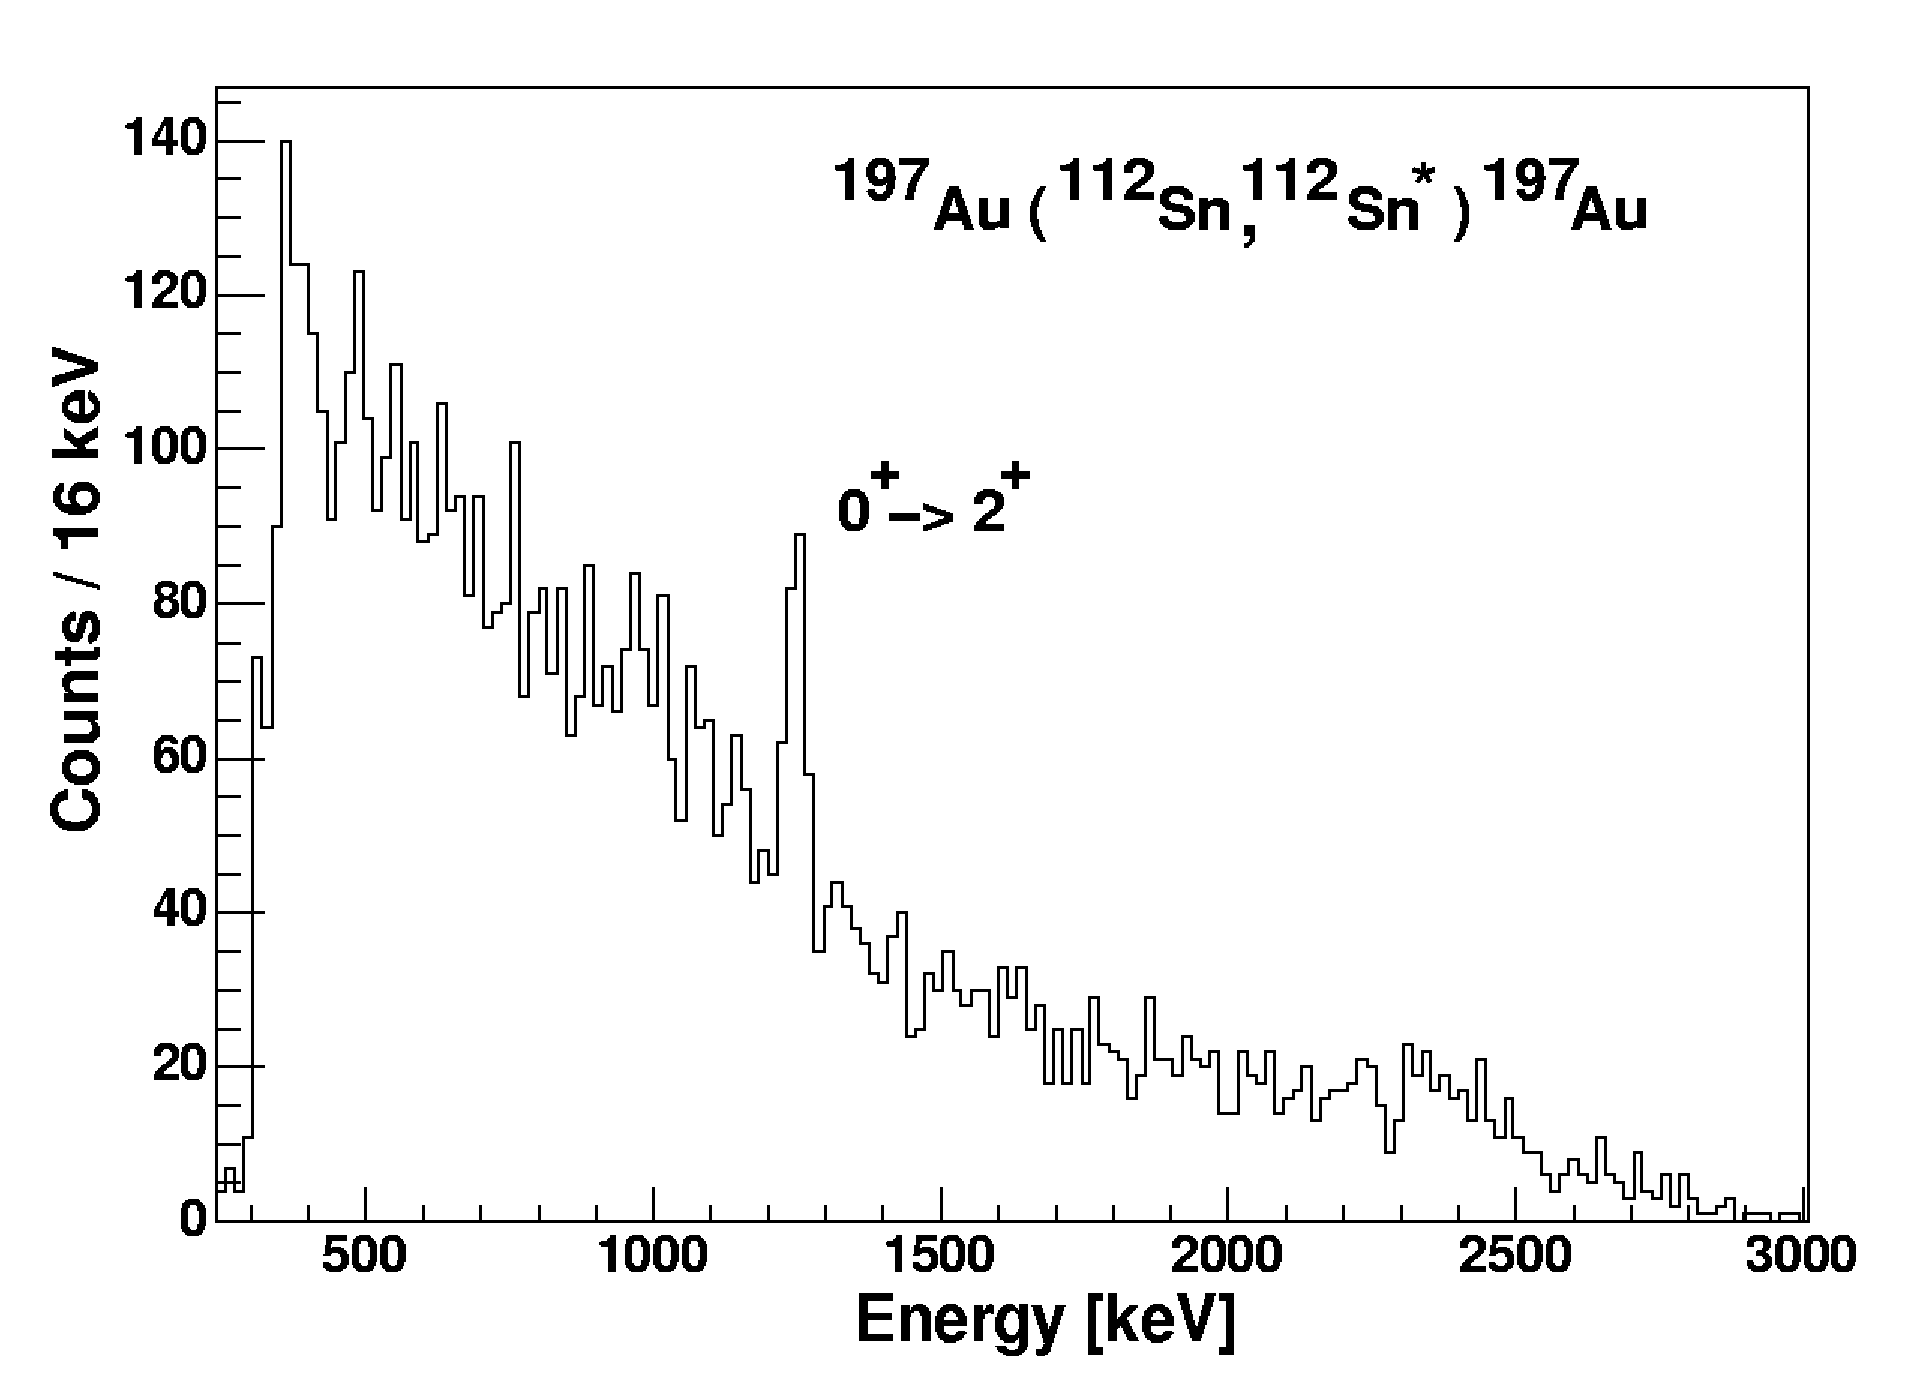
\includegraphics{fig1a.eps}}}\\
\vspace{-0.75cm}
\subfigure{%
\resizebox{0.35\textwidth}{!}{%
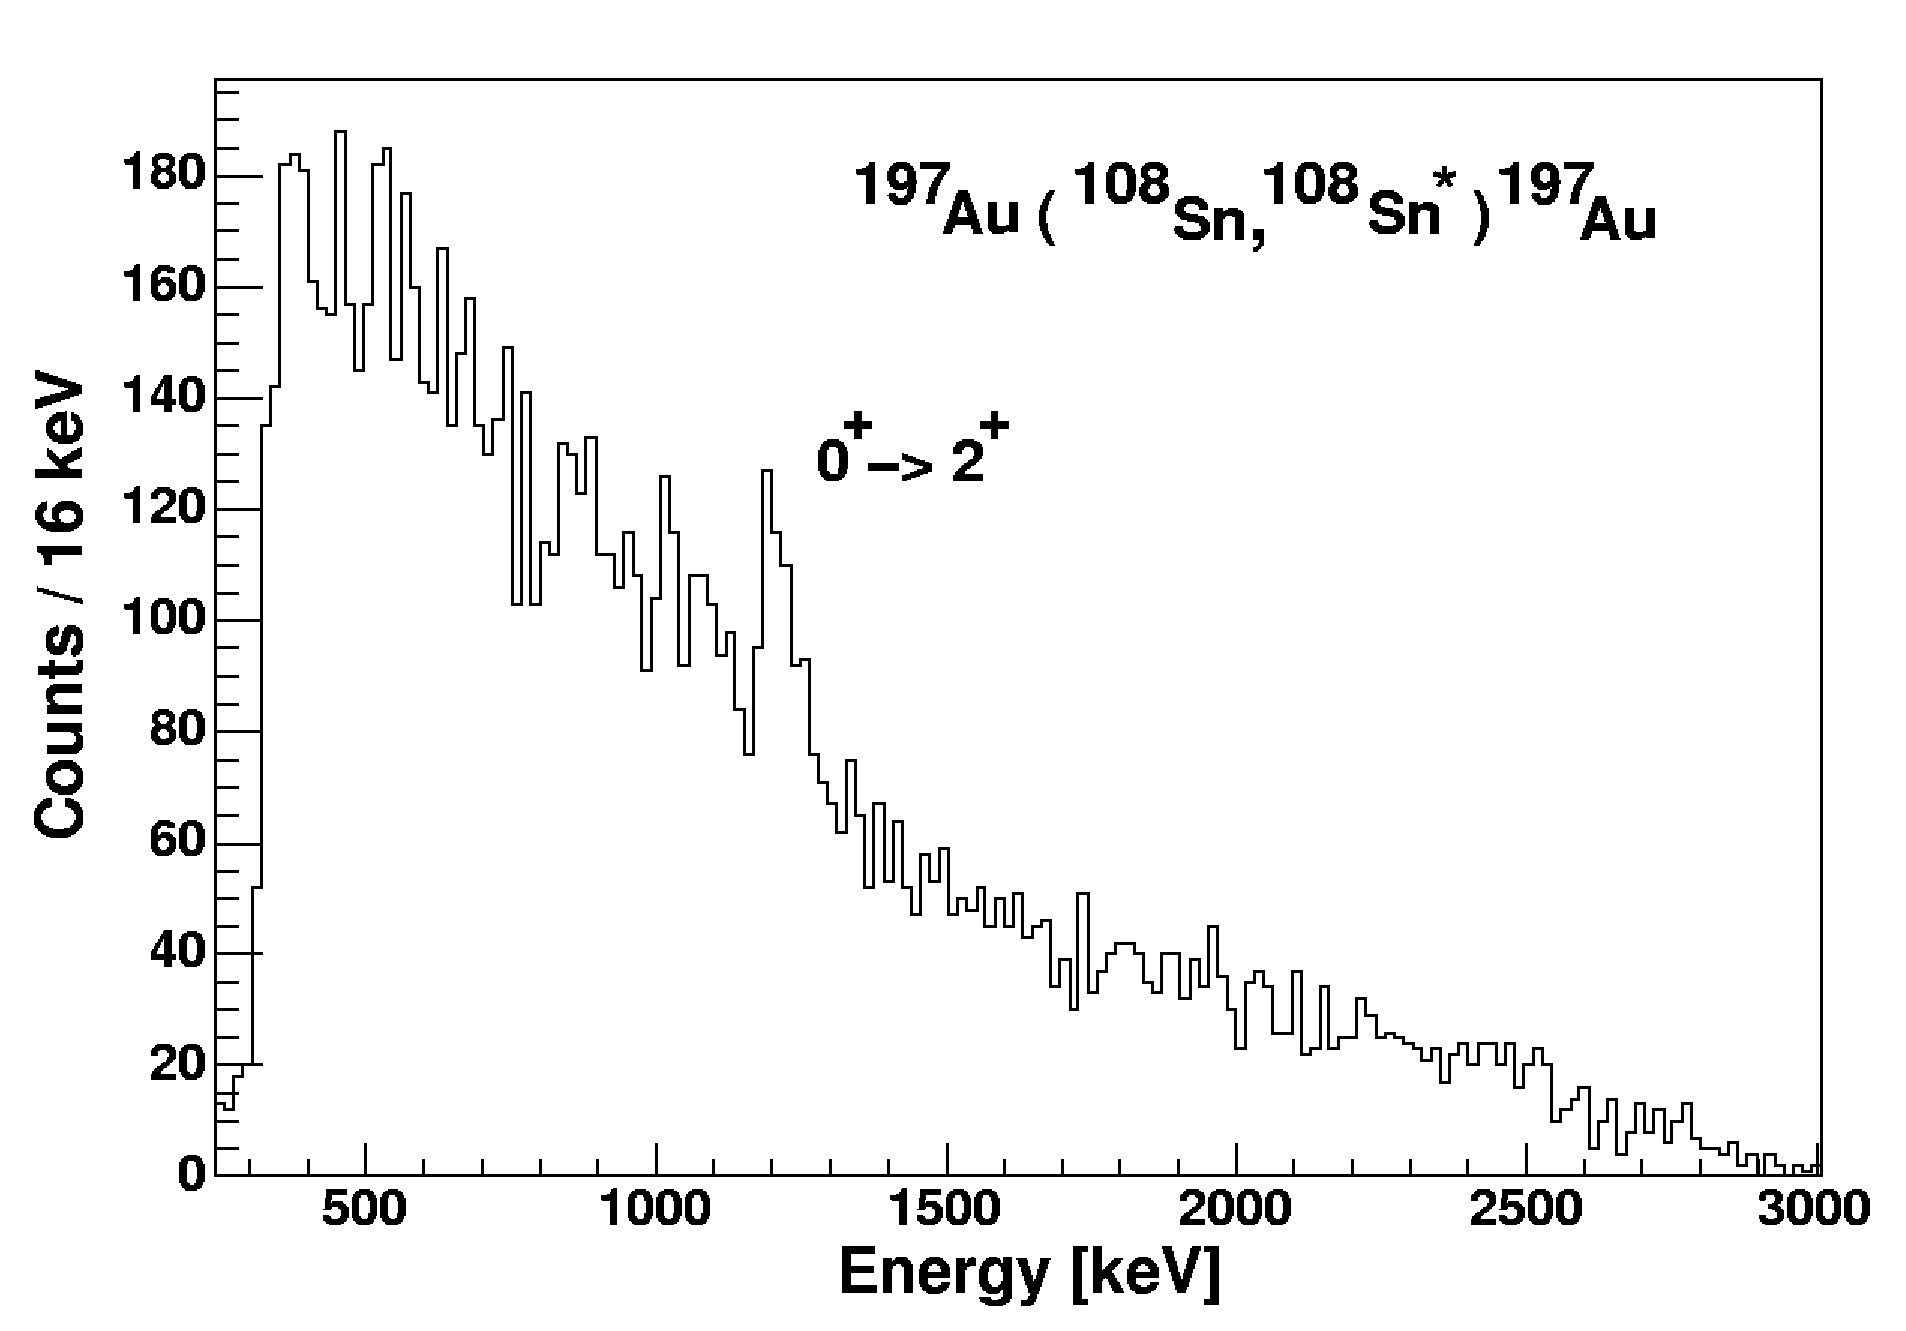
\includegraphics{fig1b.eps}}}%
\vspace{-15pt}\caption[Coulomb excitation in
$^{112,108}$Sn]{\small De-excitation $\gamma$-ray lines following
$0_{\text{g.s.}}^+ \to 2^+_1$ Coulomb excitation of the
$^{112,108}$Sn projectiles, respectively.}%
\label{fig:Sn_peaks}%
\end{figure}

The conditions applied in the data analysis to obtain the spectra
in Fig.~\ref{fig:Sn_peaks} are the following:\\
(i) fragment selection before the target with the FRS;\\
(ii) fragment selection after the target with CATE;\\
(iii) prompt gamma time \textquoteleft window\textquoteright\
($26\ \text{ns}$ wide) selection;\\
(iv) Ge-Cluster multiplicity $\text{M}_{\gamma}(\text{E}_{\gamma}
\geq 500\ \text{keV}) = 1$;\\
(v) scattering angle selection between $1^{\circ}$$-$$2^{\circ}$.\\
Having selected the fragments in the FRS, about 80$\%$ of these
events were tagged with CATE as 25$\%$ corresponding to Coulomb
excitation and the rest to fragmentation reaction channels in the
target. The intermediate-energy Coulomb excitation reaction is
predominantly an \textit{one-step process}, which implies a
$\gamma$-hit multiplicity equal to one. However, it is possible
that the de-excitation event is recorded in coincidence with
background radiation originating from either atomic processes in
the target or additional fragmentation reactions in the 1 cm thick
CATE-CsI detectors. In our case, due to a small gamma detection
efficiency ($\lesssim 1\%$), only 3$\%$ of the recorded events
correspond to a Ge-Cluster multiplicity bigger than one. For an
appropriate Coulomb excitation event selection, it was required in
the analysis that the condition of single $\gamma$-hit cluster
multiplicity is satisfied only for prompt $\gamma$ rays at
energies in excess of 500 keV (in the laboratory frame), thus
excluding non-suppressed atomic radiation.  The requested
condition on the scattering angle (calculated in the laboratory
frame) between $1^{\circ}$$-$$2^{\circ}$ corresponds approximately
to impact parameters in the range $11$ to $22\
\text{fm}$~\cite{ban05}. Below this range one expects nuclear
interactions to contribute, while above the elastic channel
dominates with an increase in the electromagnetic radiation
background. Further details on the optimization of the
aforementioned conditions may be found in~\cite{ban05}. In spite
of the strict data analysis, the spectra in
Fig.~\ref{fig:Sn_peaks} exhibit significant background even at
energies around or above 1000 keV. This background is expected
\cite{wol05} to be manly created by fragmentation of the
$^{108}$Sn/$^{112}$Sn nuclei in the thick CATE-CsI detectors,
before being stopped. The time resolution of the Ge-Clusters
($\simeq 14$ ns) is not sufficient to disentangle it from $\gamma$
rays emitted by fragments interacting with the gold target.

From the observation of the Doppler corrected $\gamma$ line
corresponding to the $0^{+}_{\text{g.s.}}$$\to$$2^{+}_{1}$
transition in $^{108}$Sn, the Coulomb excitation cross section can
be extracted, which is directly proportional to the B(E2)
value~\cite{win79}. In the analysis, effects such as
particle-$\gamma$ angular correlations, nuclear excitation or
excitations of higher-lying $2^{+}$ states (feeding contributions)
have to be considered. These data are not available due to limited
statistics. Therefore, we are presenting the experimental result
of a relative measurement of the
B(E2;0$^+_{\text{g.s.}}$$\to$2$^+_1$) value in $^{108}$Sn. The
intermediate-energy Coulomb excitation measurement performed on
$^{112}$Sn with $B(E2;0^{+}_{\text{g.s.}}\to 2^{+}_{1}) =
0.240(14)$ e$^{2}$b$^{2}$ extracted from a subbarrier Coulomb
excitation experiment~\cite{ram01}, was used as normalization.
This is justified since the two Coulomb excitation experiments
were performed under very similar conditions (\cite{ban05}). The
unknown feeding pattern is thus cancelled out (assuming similar
nuclear structure in both $^{108}$Sn and $^{112}$Sn as supported
by theory), as well as the remaining nuclear
contribution not removed by the scattering angle condition.\\
In Table~\ref{tab-1} the experimental parameters needed to
calculate the B(E2) value in $^{108}$Sn are listed. Additional
information on data-taking time and the secondary beam intensity
is given for both fragment settings.
\begin{table}[htb]
\caption{The photon yield $N_{\gamma}$, the particle flux on
target $N_{p}$, data-taking time and the counting rate
(projectiles per second) for the two $^{108,112}$Sn fragment
settings.} \label{tab-1}
\begin{tabular}[t]{ccccc}
\hline \hline
           &               &              &               &  ~~~ \\
Isotope ~~~& $N_{\gamma}$\footnotemark[1] & $N_{p}$\footnotemark[2] &  data-taking ~& ~~~~intensity\\
           &               &              &       time        &  ~~~ \\
\hline \hline
           &               &              &               &  ~~~ \\
$^{108}$Sn & 174(26) ~~~  & 15 $\times$ 10$^{7}$&  58 h   & 2480 Hz\\
           &               &              &               &  ~~~ \\
$^{112}$Sn & 106(20) ~~~  & 10 $\times$ 10$^{7}$&  33 h   & 2400 Hz\\
           &               &              &               &  ~~~ \\
\hline \hline
\end{tabular}
\footnotetext[1]{The photon yield was recorded with
$\gamma$-particle trigger.} \footnotetext[2]{The particle flux on
target was inferred from down-scaled particle-singles trigger (see
Ref.~\cite{ban05}).}
\end{table}

The B(E2;0$^+_{\text{g.s.}}$$\to$2$^+_1$) value in $^{108}$Sn was
determined as follows
\begin{displaymath}
B(E2\uparrow)_{\text{108}} = B(E2\uparrow)_{\text{112}} \times
\frac{N^{\text{108}}_{\gamma}}{N^{\text{112}}_{\gamma}} \times
\frac{N^{\text{112}}_p}{N^{\text{108}}_p} \times 0.88,
\end{displaymath}
yielding B(E2;$0^+_{\text{g.s.}}\to2^+_1)_{\text{108}} $=
0.230(57) $\text{e}^{2}\text{b}^{2}$.\\
The value $0.88$ corresponds to the ratio of the proportionality
factors between the excitation cross section and the reduced
transition probability for $^{112}$Sn and $^{108}$Sn. The
proportionality factors were calculated with the standard code
DWEIKO \cite{ber03} used for nuclear scattering at intermediate
and high energies (E$_{\text{lab}}$ $\geqslant$ 50 MeV/nucleon),
taking into account the scattering angle selection applied in the
data analysis. Because the $2^{+}_{1}$ excited states in
$^{108,112}$Sn lie close in energy, equal $\gamma$-ray
efficiencies within experimental uncertainties were considered in
the B(E2) determination.

In the following, the measured B(E2$\uparrow$) value in the
unstable $^{108}$Sn is compared to the results of two large-scale
shell model (LSSM) calculations. The first set of LSSM
calculations was performed for the tin isotopes $^{102-130}$Sn,
with a  model space for neutrons consisting of the $1d_{5/2}$,
$0g_{7/2}$, $1d_{3/2}$, $2s_{1/2}$, and $0h_{11/2}$ orbitals. Two
sets of interactions with closed shell cores $^{100}$Sn and
$^{132}$Sn were considered, following the prescription outlined in
Ref.~\cite{hjo95} and using the CD-Bonn potential for the bare
nucleon-nucleon interaction~\cite{mac96}. In the discussion here
we focus however on the results obtained with the $^{100}$Sn
closed shell core. A harmonic-oscillator basis was chosen for the
single-particle wave functions, with an oscillator energy
$\hbar\omega$ $= 8.5\ \text{MeV}$. The single-particle energies of
the chosen model space orbits are $\epsilon_{1d_{5/2}}$ $= 0.00\
\text{MeV}$, $\epsilon_{0g_{7/2}}$ $= 0.08\ \text{MeV}$,
$\epsilon_{1d_{3/2}}$ $= 1.66\ \text{MeV}$, $\epsilon_{2s_{1/2}}$
$ = 1.55\ \text{MeV}$, and $\epsilon_{0h_{11/2}}$ $= 3.55\
\text{MeV}$. The neutron effective charge used in the calculations
is $1.0e$. The results of the calculations for the energies of the
2$^+_1$ excited states and B(E2;0$^+_{\text{g.s.}}$$\to$2$^+_1$)
values are presented in the columns 3 and 5 of Table~\ref{tab-2}
together with the experimental data measured recently for the
unstable light isotope $^{108}$Sn (this work), the unstable heavy
isotopes $^{126,128,130}$Sn \cite{rad04}, and the previously
measured values for the stable isotopes $^{112-124}$Sn
\cite{ram01}.
\begin{table}[htb]
\caption{$I^\pi=2^+$ energies and E2 strengths in
$^{102-130}$Sn.}\label{tab-2}
\begin{tabular}[t]{llrll}
\hline \hline \vspace{5pt}
Isotope&~~~~~~~~~& E$_{2^{+}_{1}}$ [keV] & ~~~~~~~& B(E2$\uparrow$) [e$^2$b$^2$]   \\
\end{tabular}
\begin{tabular}{cccccc}
           & Exp.\footnotemark[1] & SM\footnotemark[2] & Exp. & SM\footnotemark[2]&
SM\footnotemark[3]   \\
\hline \hline
$^{102}$Sn & 1472.0(2) & 1647 & & 0.043 &0.044  \\
$^{104}$Sn & 1260.1(3) & 1343 & & 0.094 &  0.090\\
$^{106}$Sn & 1207.7(5) & 1231 & & 0.137 & 0.125 \\
$^{108}$Sn & 1206.1(1) & 1243 & 0.230(57)\footnotemark[4] & 0.171 &0.162  \\
$^{110}$Sn & 1211.9(2) & 1259 & & 0.192   &0.192\\
$^{112}$Sn & 1256.9(7) & 1237 & 0.240(14)\footnotemark[1] & 0.203& 0.219  \\
$^{114}$Sn & 1299.9(7) & 1208 & 0.24(5)\footnotemark[1] & 0.209  & 0.235 \\
$^{116}$Sn & 1293.6(8) & 1135 & 0.209(6)\footnotemark[1] & 0.210 & 0.241\\
$^{118}$Sn & 1229.7(2) & 1068 & 0.209(8)\footnotemark[1] & 0.208  & 0.239\\
$^{120}$Sn & 1171.3(2) & 1044 & 0.202(4)\footnotemark[1] & 0.201  & 0.228\\
$^{122}$Sn & 1140.6(3) & 1076 & 0.192(4)\footnotemark[1] & 0.184  &0.206 \\
$^{124}$Sn & 1131.7(2) & 1118 & 0.166(4)\footnotemark[1] & 0.156  & 0.174\\
$^{126}$Sn & 1141.2(4) & 1214 & 0.10(3)\footnotemark[5] & 0.118   &0.134\\
$^{128}$Sn & 1168.8(4) & 1233 & 0.073(6)\footnotemark[5] & 0.079  & 0.090\\
$^{130}$Sn & 1121.3(5) & 1191 & 0.023(5)\footnotemark[5] & 0.042  &0.047 \\
\hline \hline
\end{tabular}
\footnotetext[1]{Ref.~\cite{ram01}} \footnotetext[2]{LSSM in
$\nu$($g_{7/2},d,s,h_{11/2}$) shell model space with $^{100}$Sn
closed shell core and e$_{\text{eff}}^{\nu}=1.0e$.}
\footnotetext[3]{LSSM in $\pi$($g,d,s$) and
$\nu$($g_{7/2},d,s,h_{11/2}$) shell model space with $^{90}$Zr
closed shell core and e$_{\text{eff}}^{\nu}=0.5e$ (see text).}
\footnotetext[4]{this work} \footnotetext[5]{Ref.~\cite{rad04}}
\end{table}

The comparison between experiment and theory shows agreement for
the heavier Sn isotopes and in the case of $^{108}$Sn within error
bars. However, at a closer inspection of the light Sn isotopes,
part of the systematics seems to exceed the theoretical
predictions. In the case of the interaction inferred for a
$^{132}$Sn core, the experimental B(E2$\uparrow$) values are
reproduced with effective charges between $0.7-0.8e$ \cite{hol98}.
This indicates a different character of core excitations in the $N
= Z$ and $N > Z$ regions of the tin isotopic chain. Moreover, the
effective charges for the lighter Sn isotopes show stronger
renormalization effects, implying larger core polarization due to
particle-hole $(ph)$ excitations.

In order to shed more light on the role of core-polarization
effects, our second set of large-scale shell model calculations
includes now protons in the  $0g_{9/2}$, $0g_{7/2}$, $1d_{5/2}$,
$1d_{3/2}$ and $2s_{1/2}$ single-particle orbits as well, in
addition to neutrons in the same model space as in the first set
of calculations. The calculations allow up to 4p-4h proton core
excitations (our computational limit), and the effective charges
are set to the unscreened values $1.5e$ and $0.5e$ for protons and
neutrons, respectively. Our closed shell core is now $^{90}$Zr,
and the effective interaction, derived along the same lines as in
the previous and with the same nucleon-nucleon interaction, was
however phenomenologically adjusted to the spectroscopy of Sn
isotopes and $N = 82$ isotones, see Ref.~\cite{gni05} for more
details. As in this model space the m-scheme dimension
\cite{cau02} would be excessively large, the coupled code NATHAN
\cite{cau02} is used, which allows for a seniority truncation.
Convergence was nearly obtained for seniority $v=8$.

The experimentally observed asymmetry of the B(E2) systematics,
supported also by recent preliminary results on $^{110}$Sn
measured at REX-ISOLDE \cite{ced05}, suggests to study the role of
proton core excitations and the evolution of the Z=50 shell gap.
The proton-neutron interaction, in particular the
$\pi(0g_{9/2})-\nu(0g_{7/2}1d_{5/2}1d_{3/2}2s_{1/2})$ monopoles,
responsible for the evolution of the spectroscopy between
$^{91}$Zr and $^{101}$Sn, governs the evolution of the proton
$Z=50$ gap with the neutron filling. The tuning of the interaction
for $^{91}$Zr and $^{101}$Sn is therefore sufficient to maintain
the experimental $Z=50$ shell gap as extracted from mass
measurements.
\begin{figure}[hhh]\hspace{-0.5cm}
\centering\mbox{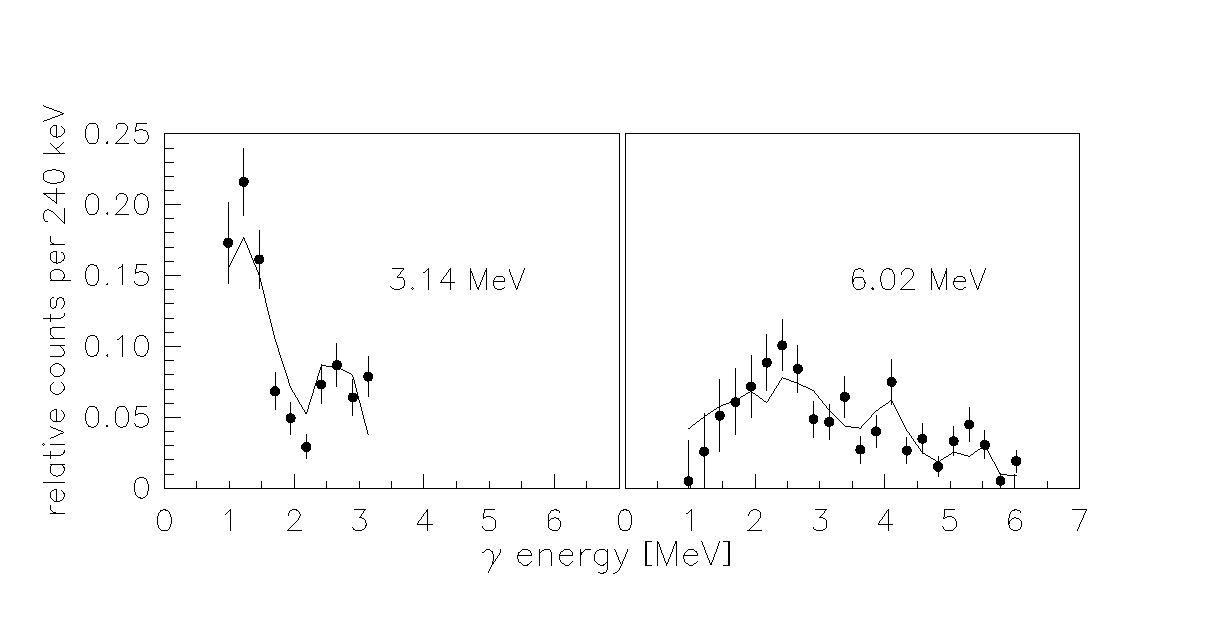
\epsfig{file=fig3.eps,width=.40\textwidth}}
\vspace{-15pt}\caption{\small Calculated evolution of the proton
ESPE with the neutron number N along the chain of Sn isotopes.}
\label{fig:ESPE}
\end{figure}
\begin{figure}[!t]\hspace{-0.5cm}
\centering\mbox{\epsfig{file=fig4_hg_ab.eps,width=0.5\textwidth}}
\vspace{-15pt}\caption{\small Comparison of measured
B(E2$\uparrow$) values with LSSM predictions by taking into
account $ph$ core excitations. The $t=0$ curve corresponds to
calculations only for the valence neutrons as active particles.
The $t=2$ curve shows the major contribution as given by proton
core excitations. The $t=4$ curves are shown for the whole tin
chain in a truncated proton model space and untruncated in the
$gds$ major shel3.}\label{fig:systematics2}
\end{figure}
This is reflected in Fig.~\ref{fig:ESPE} for the proton Effective
Single Particle Energies (ESPE), as defined in Ref. \cite{ots01},
along the tin chain. Note that the ESPEs shown are not identical
with the experimentally observed single particle states which
comprise configuration mixing. In particular, Fig.~\ref{fig:ESPE}
shows the crossing for the ESPEs of the $1d_{5/2}$ and $0g_{7/2}$
orbitals due to a strong $g_{7/2} - h_{11/2}$ proton-neutron
monopole. An equally strong $g_{9/2} - h_{11/2}$ proton-neutron
monopole is also needed that a sufficiently closed $^{132}$Sn core
is maintained.

In Fig.~\ref{fig:systematics2} the experimental B(E2) values
\cite{ban05, ram01, rad04} are compared to LSSM results for an
increasing number $t=n$ of proton np-nh excitations. The
evolutions of the B(E2) systematics presented here from the pure
neutron space to $t=4$ proton excitations are very instructive:
besides reflecting the number of interacting nucleons, the $t=0$
curve shows a slight asymmetric maximum at $N=70$, which is
shifted to $N=68$ ($t=2$) and $N=66$ ($t=4$) with increasing
number of $ph$ excitations. It should be noticed that for the
lightest Sn isotopes the calculations suffer from the strong
assumptions of an $N=50$ closure, thus the B(E2) values for
$^{102-106}$Sn are not fully trustworthy in our valence space. A
gain of 15$\%$ in the E2 strength has been estimated for
$^{106}$Sn in the $gds$ shell model space when both proton and
neutron core excitations are allowed. It is also interesting to
note that the untruncated 4p-4h proton core excitations ($t=4$
gds), listed in the last column of Table~\ref{tab-2}, show no
increase, but rather a small decrease in the B(E2) strength for
the heavy Sn isotopes in comparison to the $t=4$ calculations
truncated to the $0g_{9/2},0g_{7/2},1d_{5/2}$ orbitals, whereas
for the light ones a substantial increase is observed. For the
midshell and heavy Sn isotopes the $t=4$ calculations seem to
overestimate the E2 strength, which can be ascribed to an
ambiguity in the $\pi (0g_{9/2}) - \nu (1h_{11/2})$ monopole due
to experimental uncertainties in the $11/2^-$ states of $N=51$
isotones. A slight increase of the monopole contribution to the
interaction would enlarge the $Z=50$ shell gap in the heavier Sn
isotopes and, hence reduces the B(E2) values. These calculations
demonstrate the important role of core-polarization effects when
we break the $^{100}$Sn core and allow for proton excitations.
Starting with an effective charge of $0.5e$, one clearly sees how
the experimental B(E2) values are reached when we allow for more
proton particle-hole excitations. Without these excitations and
with neutrons only as degrees of freedom one would need neutron
effective charges in the range of $1-1.5e$ in order to explain the
experimental data. A more detailed discussion of these
calculations will be presented in a forthcoming paper
\cite{gni05}.\\

In conclusion, the B(E2;0$^+_{\text{g.s.}}$$\to$2$^{+}_1$) value
in the unstable $^{108}$Sn isotope was measured for the first time
by intermediate-energy Coulomb excitation. This is the highest-Z
nucleus studied with this method. The comparison with two
different but complementary large-scale shell model calculations
shows reasonable agreement with experiment and gives insight into
the microscopic structure of the neutron E2 polarization charge.
The evolution of proton ESPEs and the $Z=50$ shell gap with
increasing occupation of the N=50-82 major shell governs the E2
correlations related to core polarization. The experimentally
observed asymmetry can be traced back to enhanced polarization for
light Sn isotopes at $t \geq 4$ proton $ph$ excitations and/or to
neutron core excitations across the N=50 shell gap. The successful
B(E2) measurement on $^{108}$Sn at GSI opens the research path to
study with intermediate-energy
Coulomb excitation the lighter Sn isotopes towards $^{100}$Sn.\\

We thank the GSI accelerator staff for their efforts to produce a
good quality primary $^{124}$Xe beam and the DVEE division at GSI
for their support in data acquisition and Go4 software. This work
was supported by the BMBF under contracts 06MZ176 and 06-K-167.

\begin{thebibliography}{100}
\bibitem{ots01} T.~Otsuka \textit{et al.},
\Journal{\PRL}{87}{082502}{2001}.
\bibitem{gra04} H.~Grawe, in \textit{The Euroschool Lectures on Physics with Exotic Beams,
Vol.I}, Lect. Notes Phys. \textbf{651} (Springer, Berlin
Heidelberg, 2004), p. 33.
\bibitem{naz95} W.~Nazarewicz, J.~Dobaczewski, and T.R.~Werner., Physica Scripta T
\textbf{56}, 9, (1995).
\bibitem{gor97} M. G{\'o}rska \textit{et al}.,
\Journal{\PRL}{79}{2415}{1997}.
\bibitem{bla04} A.~Blazhev \textit{et al}.,
\Journal{\PRC}{69}{64304}{2004}.
\bibitem{lip98} M. Lipoglav\v{s}ek \textit{et al}.,
\Journal{\PLB}{440}{246}{1998}.
\bibitem{gor98} M. G{\'o}rska \textit{et al}., \Journal{\PRC}{58}{108}{1998}.
\bibitem{lew94} M. Lewitowicz \textit{et al}.,
\Journal{\PLB}{332}{20}{1994}.
\bibitem{sch94} R Schneider \textit{et al}.,
\Journal{\ZPA}{348}{241}{1994}.
\bibitem{ram01} S. Raman, C.W.~Nestor, and P.~Tikkanen, \Journal{\ADNDT}{78}{42}{2001}.
\bibitem{wol05} H.J. Wollersheim \textit{et al}.,
\Journal{\NIMR}{537}{637}{2005}.
\bibitem{gei92} H. Geissel \textit{et al}., \Journal{\NIMB}{70}{286}{1992}.
\bibitem{sim97} J. Simpson, \Journal{\ZPA}{358}{139}{1997}.
\bibitem{loz05} R. Lozeva \textit{et al}., \Journal{\ActaB}
{B36}{1245}{2005}.
\bibitem{ban05} A. Banu, Ph.D. thesis (2005), University of Mainz.
\bibitem{win79} A. Winther and K. Alder,
\Journal{\NPA}{A319}{518}{1979}.
\bibitem{ber03} C.A. Bertulani, C.M.~Campbell, and T.~Glasmacher,
\Journal{\CPC}{152}{317}{2003}.
\bibitem{hjo95} M. Hjorth-Jensen, T.T.S.~Kuo, and E.~Osnes,
\Journal{\PRep}{261}{125}{1995}.
\bibitem{mac96} R. Machleidt, F.~Sammarruca, and Y.~Song,
\Journal{\PRC}{53}{R1483}{1996}.
\bibitem{hol98} A. Holt, T.~Engeland, M.~Hjorth-Jensen, and E.~Osnes, \Journal{\NPA}{A634}{41}{1998}.
\bibitem{rad04} D.C. Radford \textit{et al}.,
\Journal{\NPA}{A746}{83c}{2004}.
\bibitem{tal77} I. Talmi, Proc. Int. School "Enrico Fermi",
\textit{Elementary Modes of Excitation in Nuclei}, ed. A.~Bohr and
R.A.~Broglia (North Holland, Amsterdam, 1977) p.352.
\bibitem{gni05} A. Gniady \textit{et al}. (to be published).
\bibitem{cau02} E. Caurier and G.~Mart{\'i}nez-Pinedo, \Journal{\NPA}{A704}{60c}{2002}.
\bibitem{ced05} J. Cederk{\"a}ll \textit{et al}. (to be published).

\end{thebibliography}
\end{document}
